\documentclass[
	a4paper,
	oneside,
	BCOR = 10mm,
	DIV = 12,
	12pt,
	headings = normal,
]{scrartcl}

%%% Length calculations
\usepackage{calc}
%%%

%%% Support for color
\usepackage{xcolor}
\definecolor{lightblue}{HTML}{03A9F4}
\definecolor{red}{HTML}{F44336}
%%%

%%% Including graphics
\usepackage{graphicx}
%%%

%%% Font selection
\usepackage{fontspec}

\setromanfont{STIX Two Text}[
	SmallCapsFeatures = {LetterSpace = 8},
]

\setsansfont{IBM Plex Sans}[
	Scale = MatchUppercase,
]

\setmonofont{IBM Plex Mono}[
	Scale = MatchUppercase,
]
%%%

%%% Math typesetting
\usepackage{amsmath}

\usepackage{unicode-math}
\setmathfont{STIX Two Math}

\usepackage{IEEEtrantools}
%%%

%%% List settings
\usepackage{enumitem}
\setlist[enumerate]{
	label*      = {\arabic*.},
	leftmargin  = *,
	labelindent = \parindent,
	topsep      = 1\baselineskip,
	parsep      = 0\baselineskip,
	itemsep     = 1\baselineskip,
	noitemsep, % override itemsep
}

\setlist[itemize]{
	label*      = {—},
	leftmargin  = *,
	labelindent = \parindent,
	topsep      = 1\baselineskip,
	parsep      = 0\baselineskip,
	itemsep     = 1\baselineskip,
	noitemsep, % override itemsep
}

\setlist[description]{
	font        = {\rmfamily\upshape\bfseries},
	topsep      = 1\baselineskip,
	parsep      = 0\baselineskip,
	itemsep     = 0\baselineskip,
}

%%%

%%% Structural elements typesetting
\setkomafont{pagenumber}{\rmfamily\upshape}
\setkomafont{disposition}{\rmfamily\bfseries}

% Sectioning
\RedeclareSectionCommand[
	beforeskip = -1\baselineskip,
	afterskip  = 1\baselineskip,
	font       = {\normalsize\bfseries\scshape},
]{section}

\RedeclareSectionCommand[
	beforeskip = -1\baselineskip,
	afterskip  = 1\baselineskip,
	font       = {\normalsize\bfseries\itshape},
]{subsection}

\RedeclareSectionCommand[
	beforeskip = -1\baselineskip,
	afterskip  = 1\baselineskip,
	font       = {\normalsize\bfseries},
]{subsubsection}

\RedeclareSectionCommand[
	beforeskip = -1\baselineskip,
	afterskip  = -0.5em,
	font       = {\normalsize\mdseries\scshape\addfontfeatures{Letters = {UppercaseSmallCaps}}},
]{paragraph}
%%%

%%% Typographic enhancements
\usepackage{microtype}
%%%

%%% Language-specific settings
\usepackage{polyglossia}
\setmainlanguage{ukrainian}
\setotherlanguages{english}
%%%

%%% Captions
\usepackage{caption}
\usepackage{subcaption}

%\DeclareCaptionLabelFormat{closing}{#2)}
%\captionsetup[subtable]{labelformat = closing}

%\captionsetup[subfigure]{labelformat = closing}

\captionsetup[table]{
	aboveskip = 0\baselineskip,
	belowskip = 0\baselineskip,
}

\captionsetup[figure]{
	aboveskip = 1\baselineskip,
	belowskip = 0\baselineskip,
}

\captionsetup[subfigure]{
	labelformat = simple,
	labelformat = brace,
}
%%%

%%% Hyphenated ragged typesetting
\usepackage{ragged2e}
%%%

%%% Table typesetting
\usepackage{booktabs}
\usepackage{longtable}

\usepackage{multirow}

\usepackage{array}
\newcolumntype{v}[1]{>{\RaggedRight\arraybackslash\hspace{0pt}}p{#1}}
\newcolumntype{b}[1]{>{\Centering\arraybackslash\hspace{0pt}}p{#1}}
\newcolumntype{n}[1]{>{\RaggedLeft\arraybackslash\hspace{0pt}}p{#1}}
%%%

%%% Drawing
\usepackage{tikz}
\usepackage{tikzscale}
\usetikzlibrary{positioning}
\usetikzlibrary{arrows.meta} % Stealth arrow tips
%%%

%%% SI units typesetting
\usepackage{siunitx}
\sisetup{
	output-decimal-marker = {,},
	exponent-product      = {\cdot},
	inter-unit-product    = \ensuremath{{} \cdot {}},
	per-mode              = symbol,
}
%%%

%%% Framing code listings
\usepackage{tcolorbox}
\tcbuselibrary{breakable}
\tcbuselibrary{minted}
\tcbuselibrary{skins}

\newtcblisting[
	auto counter, 
	list inside, 
	number within = section,
]{listingpython}[3][]{%
	minted language = python,
	minted style    = bw,
	minted options  = {
		linenos,
		tabsize = 4,
		breaklines,
		breakanywhere,
		fontsize = \footnotesize,
	},
	empty,
	sharp corners,
	coltitle = black,
	borderline horizontal = {1pt}{0pt}{black},
	titlerule = {0.5pt},
	titlerule style = {
		black,
	},
	toptitle = 0.3em,
	bottomtitle = 0.3em,
	before skip      = \intextsep,
	after  skip      = \intextsep,
	title            = {Лістинг \thetcbcounter: #2},
	list entry       = {\protect\numberline{\thetcbcounter}#2},
	left = 0em,
	right = 0em,
	%
	listing only,
	breakable,
	%
	label = {#3},
	%
	#1
}

\newtcbinputlisting[auto counter, list inside, number within = section]{\inputpython}[4][]{%
	minted language = python,
	minted style    = bw,
	minted options  = {
		linenos,
		tabsize = 4,
		breaklines,
		breakanywhere,
		fontsize = \footnotesize,
	},
	empty,
	sharp corners,
	coltitle = black,
	borderline horizontal = {1pt}{0pt}{black},
	titlerule = {0.5pt},
	titlerule style = {
		black,
	},
	toptitle = 0.3em,
	bottomtitle = 0.3em,
	before skip      = \intextsep,
	after  skip      = \intextsep,
	title            = {Лістинг \thetcbcounter: #3},
	list entry       = {\protect\numberline{\thetcbcounter}#3},
	left = 0em,
	right = 0em,
	%
	listing file={#2},
	listing only,
	breakable,
	%
	label = {#4},
	%
	#1
}

% Customize minted
\usepackage{minted}
\setmintedinline{
	style = bw,
	breaklines,
}

% Customize minted line numbers
\renewcommand{\theFancyVerbLine}{\ttfamily\scriptsize\arabic{FancyVerbLine}}

%%%

%%% Links and hyperreferences
\usepackage{hyperref}
\hypersetup{
	bookmarksnumbered = true,
	colorlinks      = false,
	linkbordercolor = red,
	urlbordercolor  = lightblue,
	pdfborderstyle  = {/S/U/W 1.5},
}
%%%

%%% Length adjustment

% Set baselineskip, default is 14.5 pt
\linespread{1.068966} % ~15.5 pt
\setlength{\emergencystretch}{1em}
\setlength{\parindent}{1.5em}
\newlength{\gridunitwidth}
\setlength{\gridunitwidth}{\textwidth / 12}
%%%

%%% Custom commands
\newcommand{\allcaps}[1]{{\addfontfeatures{LetterSpace = 8, Kerning = Off}#1}}
\newcommand{\filename}[1]{\texttt{#1}}
\newcommand{\progname}[1]{\texttt{#1}}
\newcommand{\modulename}[1]{\texttt{#1}}
%%%

%%% Custom math commands
\newcommand{\longvar}[1]{\mathit{#1}}
%%%

\begin{document}

\begin{titlepage}
		\begin{center}
			Міністерство освіти і науки України\\
			Національний авіаційний університет\\
			Навчально-науковий інститут комп'ютерних інформаційних технологій\\
			Кафедра комп'ютеризованих систем управління

			\vspace{\fill}
				Лабораторна робота №4\\
				з~дисципліни «Імітаційне моделювання»\\
				на~тему «Моделювання неперервних випадкових величин»\\

			\vspace{\fill}

			\begin{flushright}
				Виконав:\\
				студент \allcaps{ННІКІТ}\\
				групи СП-325\\
				Клокун В.\,Д.\\
				Перевірила:\\
				Марченко Н.\,Б.
			\end{flushright}

			Київ 2019
		\end{center}
	\end{titlepage}

	\section{Мета роботи}
		Ознайомитись з~методом оберненої функції імітації неперервних випадкових величин; побудувати імітаційну модель отримання системи неперервних випадкових величин (СНВВ).

	\section{Хід роботи}
		Для виконання роботи поставлені такі завдання:
		\begin{enumerate}
			\item Відповідно до варіанту завдання знайти функцію вигляду $X = F^{-1}(\xi)$, використовуючи метод оберненої функції.
			\item Побудувати імітаційну модель отримання системи неперервних випадкових величин (СНВВ), що мають рівномірний розподіл на проміжку $[0; 1]$ (використати генератор псевдовипадкових чисел).
			\item На основі СНВВ в створеній програмі побудувати графік функції розподілу~$F(x)$ неперервної випадкової величини~$X$ за методом оберненої функції.
			\item Знайти ймовірність того, що неперервна випадкова величина~$X$ прийме значення, яке належить інтервалу~$[a; b]$.
		\end{enumerate}

		\paragraph{Завдання за варіантом} Функція $F(x) = x^3$, границі інтервалу: $a = \num{0.5}, b = \num{0.9}$.

		Під час виконання роботи була розроблена імітаційна модель для виконання поставлених завдань і реалізована у вигляді відповідного програмного засобу (ліст.~\ref{lst:full-solution}). Реалізований програмний засіб був запущений на~моделювання і~надавав стабільний і~очікуваний результат~(рис.~\ref{fig:program_scr}). В результаті програма будує графік функції ймовірностей~(рис.~\ref{fig:pmf}).

		\begin{figure}[!htbp]
			\centering
			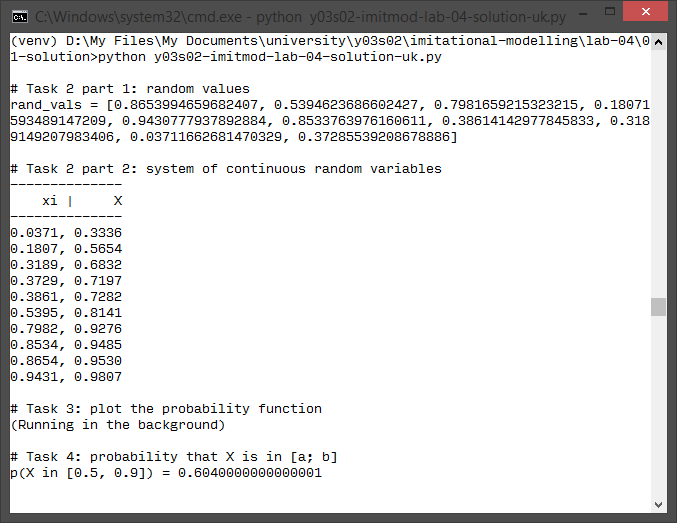
\includegraphics[height = 10\baselineskip]{./assets/y03s02-imitmod-lab-04-p00.png}
			\caption{Результат роботи програми: вікно терміналу}
			\label{fig:program_scr}
		\end{figure}
		
		\begin{figure}[!htbp]
			\centering
			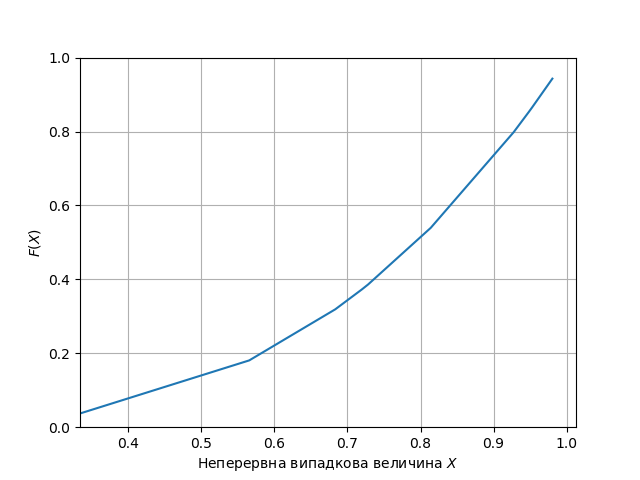
\includegraphics[height = 14\baselineskip]{./assets/y03s02-imitmod-lab-04-p01.png}
			\caption{Графік функції ймовірностей}
			\label{fig:pmf}
		\end{figure}

		\section{Висновок}
			Виконуючи дану лабораторну роботу, ми ознайомились з~методом оберненої функції імітації неперервних випадкових величин; побудували імітаційну модель отримання системи неперервних випадкових величин (СНВВ).

		\appendix
		\section{Повний початковий код програмної реалізації}
		\label{sec:full-listing}
			\begin{listingpython}[toprule = 0pt, bottomrule = 0pt]{Повний початковий код програмної реалізації}{lst:full-solution}
#!/usr/bin/env python3
# -*- coding: utf-8 -*-
import math
import random
import matplotlib.pyplot as plt
import multiprocessing as mp


def split_list_of_points(lofp):
    """
    Розділяє список точок у вигляді [(x1, y1), (x2, y2), (x3, y3), ...]
    у два кортежі: x = (x1, x2, x3, ...), y = (y1, y2, y3, ...)
    """
    x, y = zip(*lofp)
    return x, y


def calc_x_in_ab_prob(f, a, b):
    r"""
    Обчислює ймовірність того, що значення зі списку `X` попадають в інтервал
    [a, b]

    :param f: початкова, не обернена функція, за якою обчислюється ймовірність
        попадання в інтервал
    :type func:
    :param a: нижня границя інтервалу (включно)
    :type float:
    :param b: верхня границя інтервалу (включно)
    :type float:
    :returns: ймовірність того, що значення попадають в інтервал $[a, b]$
    :rtype float:
    """
    # Знаходимо менше і більше значення, щоб уникнути зворотних інтервалів
    lesser_val, greater_val = sorted([a, b])
    return f(greater_val) - f(lesser_val)


def plot_prob_func(X, xi, xlabel=r'$X$', ylabel=r'$\xi$'):
    r""" Будує графік функції ймовірностей

    :param X: значення $X$ — ймовірності
    :type X: list
    :param xi: значення $\xi$ — значення, отримані з генератора
        псевдовипадкових чисел
    :type xi: list
    :param xlabel: підпис для осі абсцис
    :type str:
    :param ylabel: підпис для осі ординат
    :type str:
    """
    fig = plt.figure(1)

    ax = fig.add_subplot(111)
    ax.plot(X, xi)
    ax.set_xlabel(xlabel)
    ax.set_ylabel(ylabel)
    # На осі OX знаходяться значення випадкової змінної, тому для наочності
    # обмежуватимемо лише мінімальним значенням
    ax.set_xlim(min(X), None)
    # На осі OY знаходяться значення ймовірності, тому для наочності завжди
    # обмежуватимемо інтервалом [0.0, 1.0]
    ax.set_ylim(0.0, 1.0)
    plt.grid()
    plt.show()
    return


def run_lab(parent_func, inverted_func, a, b, rand_count=50):
    """
    Запускає завдання лабораторної роботи на виконання

    :param parent_func: початкова функція, задана в завданні на роботу
    :type func:
    :param inverted_func: обернена функція, обчислена власноруч
    :type func:
    :param a: нижня границя інтервалу (включно)
    :type float:
    :param b: верхня границя інтервалу (включно)
    :type float:
    :param rand_count: кількість випадкових значень, які мають бути згенеровані
        для системи неперервних випадкових величин
    :type int:
    """
    # Завдання 2: створити RAND_COUNT випадкових значень, рівномірно
    # розподілених на інтервалі [0.0, 1.0)
    print('\n# Task 2 part 1: random values')

    rand_vals = [random.random() for _ in range(rand_count)]

    print('rand_vals = {}'.format(rand_vals))

    # Створити систему неперервних випадкових змінних, такого вигляду
    # (<випадкова змінна>, <значення оберненої функції для випадкової змінної>)
    print('\n# Task 2 part 2: system of continuous random variables')
    system_crv = sorted([(val, inverted_func(val)) for val in rand_vals])

    # Вивести заголовок для системи неперервних випадкових змінних
    print('{:->14}'.format(''))
    print('{:>6} |{:>6}'.format('xi', 'X'))
    print('{:->14}'.format(''))

    # Print xi, X values in the system
    # Вивести значення $\xi$, $X$ із СНВВ
    for xi, X in system_crv:
        print('{:.4f}, {:.4f}'.format(xi, X))

    xi, X = split_list_of_points(system_crv)

    # Завдання 3: побудувати графік функції ймовірностей
    print('\n# Task 3: plot the probability function'
          '\n(Running in the background)')

    # Create a process for plotting the function
    # Створюємо процес для побудови графіку функції
    p = mp.Process(
        target=plot_prob_func,
        args=(X, xi,
              r'Неперервна випадкова величина $X$',
              r'$F(X)$')
    )
    p.start()  # Запускаємо створений процес фоном

    # Завдання 4: визначити ймовірність, що величини з $X$ попадають в інтервал
    # $[a, b]$
    print('\n# Task 4: probability that X is in [a; b]')
    p = calc_x_in_ab_prob(parent_func, a, b)
    print('p(X in [{}, {}]) = {}'.format(a, b, p))


def main():
    # Оголошуємо параметри, дані у завданні варіанта
    def parent_func(x): return x**3
    a, b = 0.5, 0.9

    # Завдання 1: визначити обернену функцію
    #
    # \xi = x^3
    # \xi^{1/3} = x
    # x = \xi^{1/3}
    def inv_func(x): return x**(1/3)

    # Запустити моделювання із заданими у варіанті параметрами та 100
    # випадковими величинами
    run_lab(parent_func, inv_func, a, b, rand_count=10)


if __name__ == '__main__':
    main()
			\end{listingpython}

\end{document}

